\chapter{Ombre sulla vittoria}

Sono le sette del mattino, il sole è già sorto e le casalinghe hanno iniziato le prime pulizie.  
Sono arrivate delle artiste e nei paraggi stanno preparando gli intonaci per le loro \emph{street art}.  
Giovanni ha dormito fuori insieme al vagabondo.  
Ippa è sotto la rete, ma esce e punta i rovi di cinta.  
Le orecchie sono tese.  
Qualcuno sta penetrando nel convitto.

\par\medskip
«Saranno le artiste che cercano un posto esotico per le loro creazioni.  
Dai Ippa abbaia, così scappano e non vengono a romperci l’anima.»

\par\medskip
I latrati di Ippa non vanno a vuoto e sono risposti da un altro latrato.  
Giovanni lo ha già riconosciuto.  
Dal tunnel vegetale escono Laura, Valentina, Alice che ha Rocky al guinzaglio e Caterina che porta una torta.

\par\medskip
«Buongiorno, siamo passati a salutarvi.»\\
«Ragazze, buongiorno. Vedo che non venite a mani vuote.»

\par\medskip
Giovanni si alza e insieme a Ippa si avvicina alla tetraginia.

\par\medskip
«Abbiamo portato la colazione.»\\
«Sì, è una crostata.» Valentina precisa bene.\\
«Bisogna chiamare Luca. Il bambino che avete aiutato.»\\
«Non sono un bambino.»

\par\medskip
Luca sbuca dalle scale antincendio coperto ancora solo da un asciugamano.  
Dallo zainetto Caterina prende una stuoia da picnic, una tovaglia, piattini e bicchieri e apparecchia per la colazione.  
La crostata deve essere buona perché sparisce quasi tutta in pochi minuti insieme al succo di frutta.

\par\medskip
Giovanni cerca un tovagliolo e tastando incontra la mano di Caterina.

\par\medskip
«E il tuo viaggio?»\\
«Non sono più sicura di voler partire.»\\
«Avevo capito che fosse importante.»\\
«Lo sarebbe, ma forse non è la cosa giusta da fare.»

\par\medskip
Giovanni ascolta Caterina che continua a parlare.  
Parla tanto.  
Rocky e Ippa si rincorrono nei pochi metri quadri di erba senza penetrare tra i cespugli.  
Le casalinghe osservano il gruppo dalla finestra del secondo piano.

\par\medskip
Fin qui, tutto bene.

\par\medskip
\begin{center}
  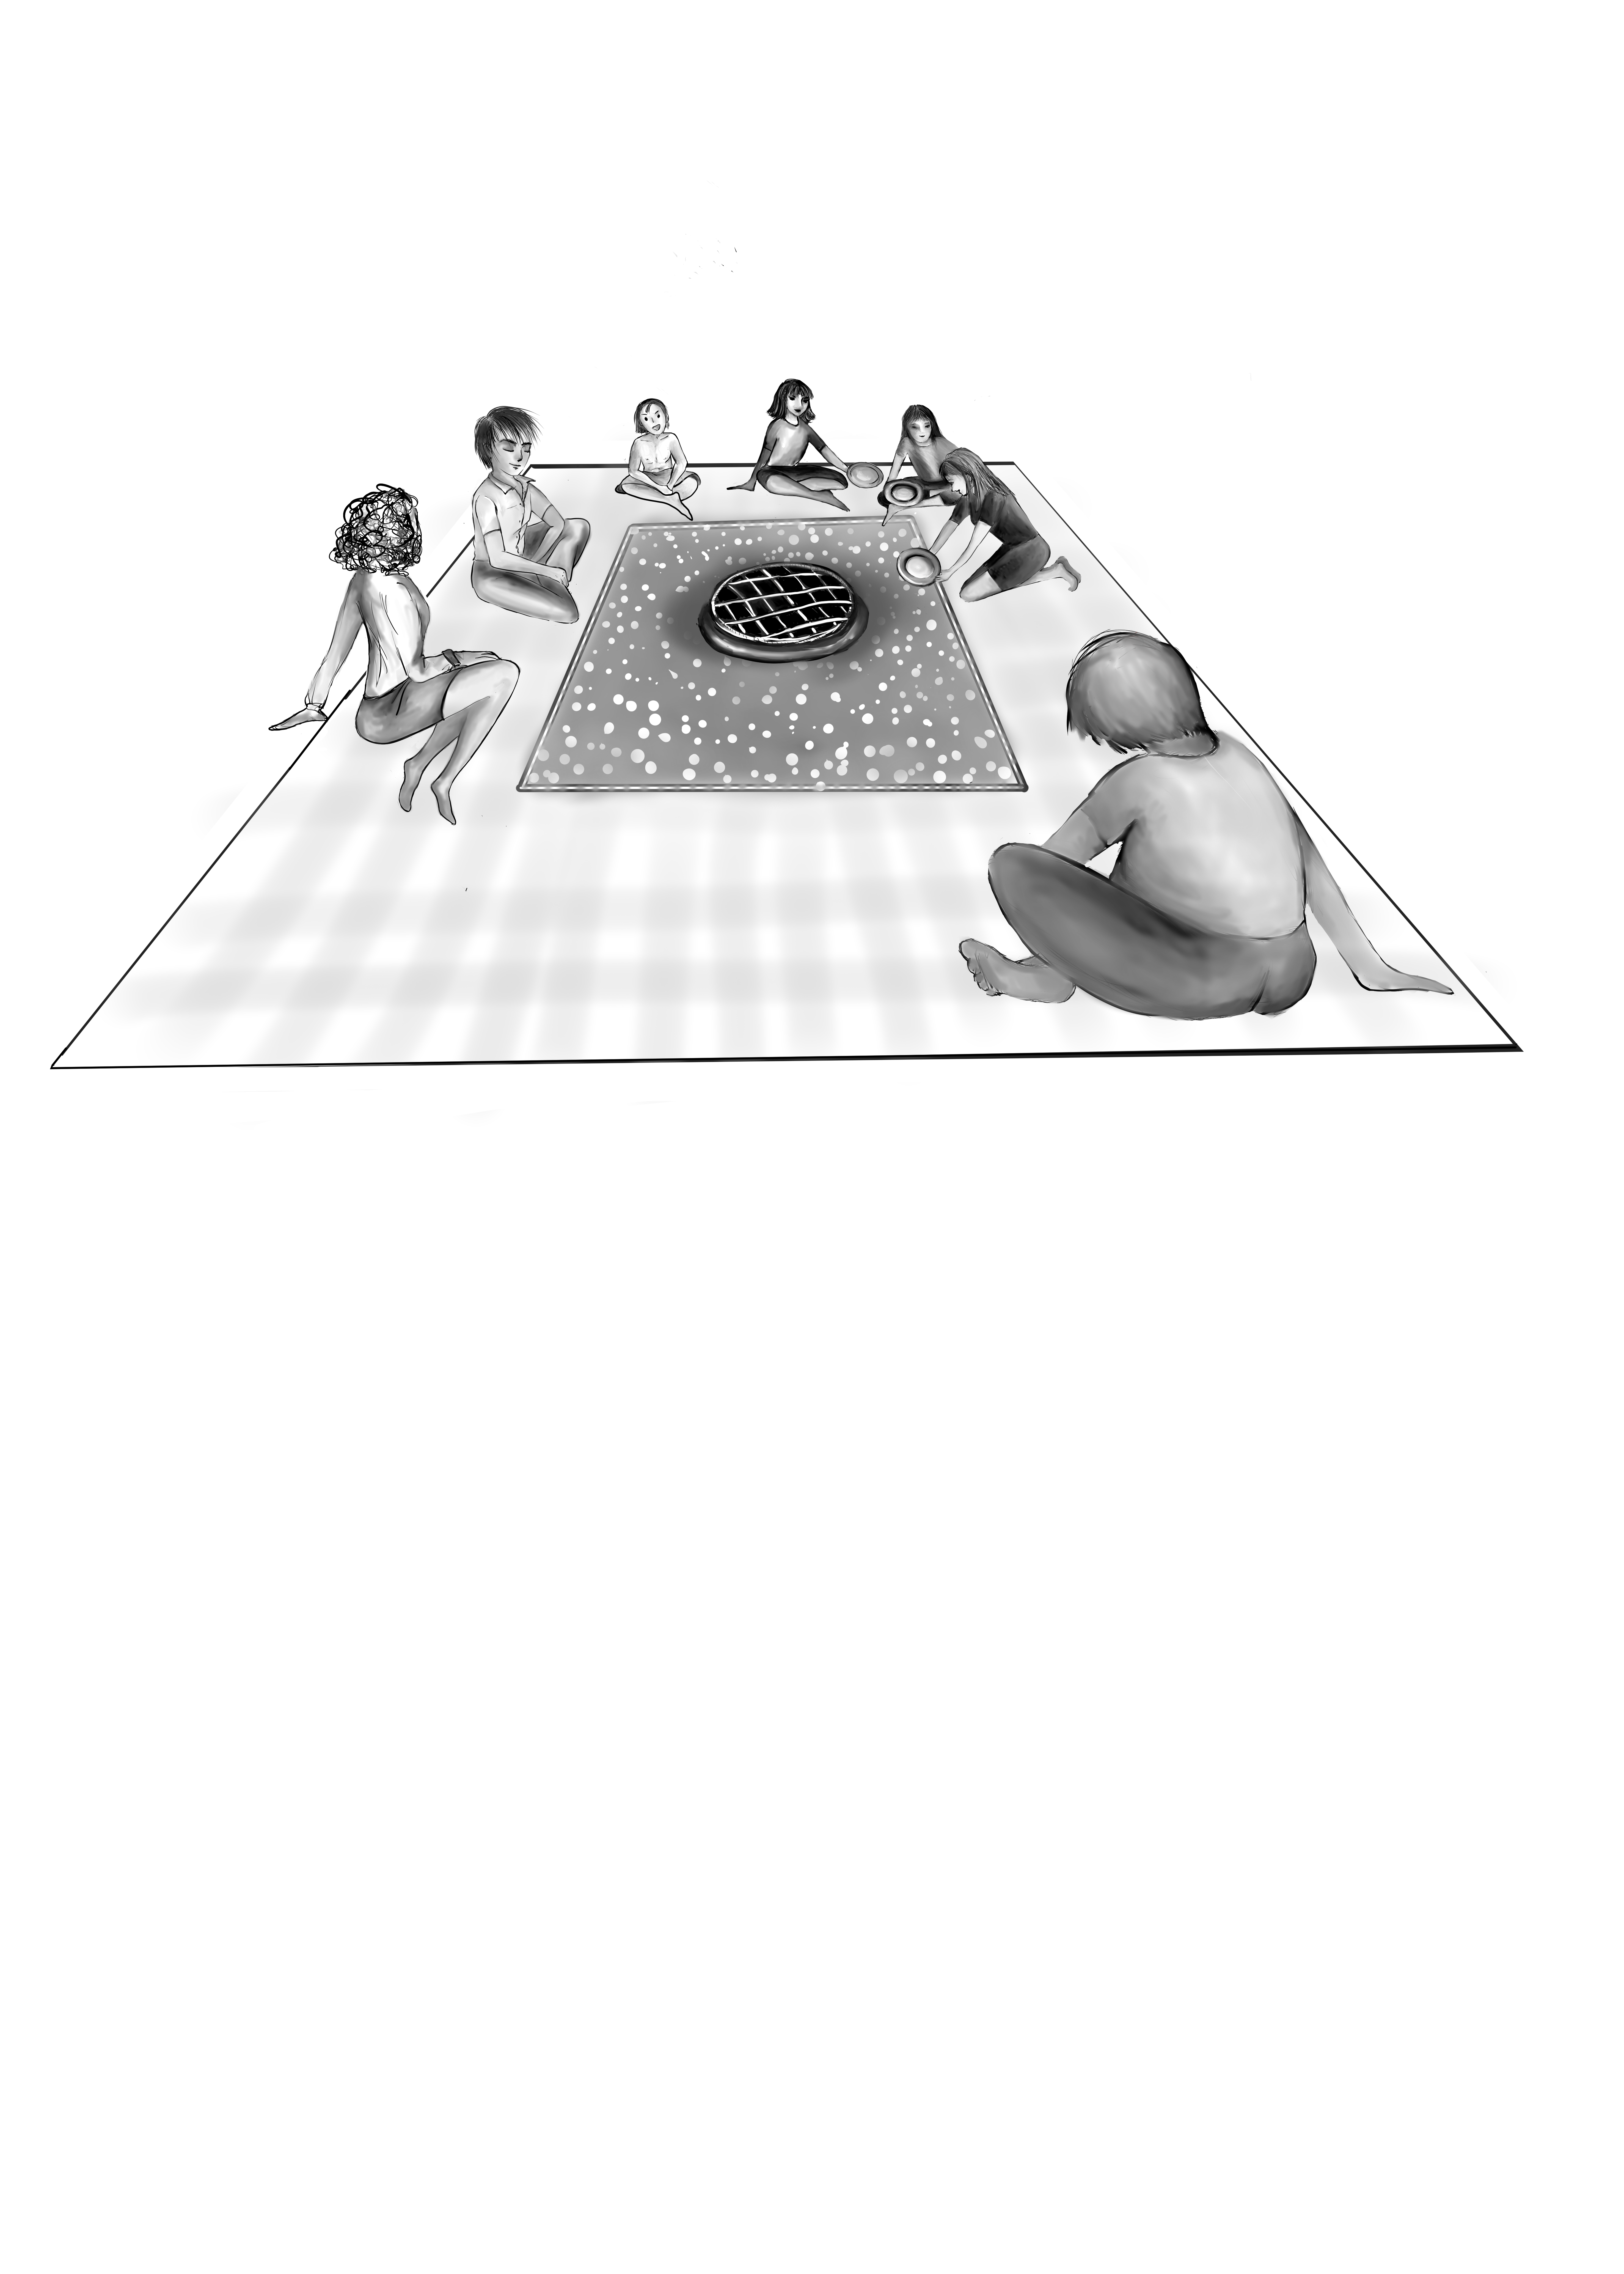
\includegraphics[width=0.9\linewidth]{picnic senza sfondo.png}
\end{center}
